%%%%%%%%%%%%%%%%%%%%%%%%%%%%%%%%%%%%%%%%%
% Short Sectioned Assignment
% LaTeX Template
% Version 1.0 (5/5/12)
%
% This template has been downloaded from:
% http://www.LaTeXTemplates.com
%
% Original author:
% Frits Wenneker (http://www.howtotex.com)
%
% License:
% CC BY-NC-SA 3.0 (http://creativecommons.org/licenses/by-nc-sa/3.0/)
%
%%%%%%%%%%%%%%%%%%%%%%%%%%%%%%%%%%%%%%%%%

%----------------------------------------------------------------------------------------
%	PACKAGES AND OTHER DOCUMENT CONFIGURATIONS
%----------------------------------------------------------------------------------------

\documentclass[paper=letter, fontsize=12pt]{scrartcl} % Letter paper and 11pt font size

\usepackage[T1]{fontenc} % Use 8-bit encoding that has 256 glyphs
\usepackage{fourier} % Use the Adobe Utopia font for the document - comment this line to return to the LaTeX default
\usepackage[english]{babel} % English language/hyphenation
\usepackage{amsmath,amsfonts,amsthm} % Math packages
\usepackage{blkarray}
\usepackage{tikz}
\usetikzlibrary{calc,trees,positioning,arrows,chains,shapes.geometric,%
  decorations.pathreplacing,decorations.pathmorphing,shapes,%
  matrix,shapes.symbols}

\tikzset{
  >=stealth',
  punktchain/.style={
    rectangle,
    rounded corners,
    % fill=black!10,
    draw=black, very thick,
    text width=10em,
    minimum height=3em,
    text centered,
    on chain
  },
  line/.style={draw, thick, <-},
  element/.style={
    tape,
    top color=white,
    bottom color=blue!50!black!60!,
    minimum width=8em,
    draw=blue!40!black!90, very thick,
    text width=10em,
    minimum height=3.5em,
    text centered,
    on chain
  },
  every join/.style={->, thick,shorten >=1pt},
  decoration={brace},
  tuborg/.style={decorate},
  tubnode/.style={midway, right=2pt},
}

\usepackage{sectsty} % Allows customizing section commands
\allsectionsfont{\centering \normalfont\scshape} % Make all sections centered, the default font and small caps

\usepackage{fancyhdr} % Custom headers and footers
\pagestyle{fancyplain} % Makes all pages in the document conform to the custom headers and footers
\fancyhead{} % No page header - if you want one, create it in the same way as the footers below
\fancyfoot[L]{} % Empty left footer
\fancyfoot[C]{} % Empty center footer
\fancyfoot[R]{\thepage} % Page numbering for right footer
\renewcommand{\headrulewidth}{0pt} % Remove header underlines
\renewcommand{\footrulewidth}{0pt} % Remove footer underlines
\setlength{\headheight}{13.6pt} % Customize the height of the header
\linespread{1.5}
\numberwithin{equation}{section} % Number equations within sections (i.e. 1.1, 1.2, 2.1, 2.2 instead of 1, 2, 3, 4)
\numberwithin{figure}{section} % Number figures within sections (i.e. 1.1, 1.2, 2.1, 2.2 instead of 1, 2, 3, 4)
\numberwithin{table}{section} % Number tables within sections (i.e. 1.1, 1.2, 2.1, 2.2 instead of 1, 2, 3, 4)

\setlength\parindent{0pt} % Removes all indentation from paragraphs - comment this line for an assignment with lots of text

\newcommand{\matx}[1] {
\begin{bmatrix}
  #1 \\
\end{bmatrix}
}

\newcommand{\matxx}[2] {
\begin{bmatrix}
  #1 \\
  #2 \\
\end{bmatrix}
}

\newcommand{\matxxx}[3] {
\begin{bmatrix}
  #1 \\
  #2 \\
  #3 \\
\end{bmatrix}
}

\newcommand{\matxxxx}[4] {
\begin{bmatrix}
  #1 \\
  #2 \\
  #3 \\
  #4 \\
\end{bmatrix}
}
\newcommand{\matxxxxx}[5] {
\begin{bmatrix}
  #1 \\
  #2 \\
  #3 \\
  #4 \\
  #5 \\
\end{bmatrix}
}

\newcommand{\matxxxxxx}[6] {
\begin{bmatrix}
  #1 \\
  #2 \\
  #3 \\
  #4 \\
  #5 \\
  #6 \\
\end{bmatrix}
}

\newcommand{\arrow}[1] {\xrightarrow[]{\text{#1}}}

%----------------------------------------------------------------------------------------
%	TITLE SECTION
%----------------------------------------------------------------------------------------

\newcommand{\horrule}[1]{\rule{\linewidth}{#1}} % Create horizontal rule command with 1 argument of height

\title{
\normalfont \normalsize
\textsc{Linear Algebra} \\ [25pt] % Your university, school and/or department name(s)
\horrule{0.5pt} \\[0.4cm] % Thin top horizontal rule
\huge A relationship between Linear Algebra and Machine Learning \\
\horrule{2pt} \\[0.5cm] % Thick bottom horizontal rule
}

\author{Yong Hoon Do, Sojung Kim} % Your name

\date{\normalsize\today} % Today's date or a custom date

\begin{document}

\maketitle % Print the title

%----------------------------------------------------------------------------------------
%	Machine Learning
%----------------------------------------------------------------------------------------
\section{What is Machine Learning}

Machine learning is defined as a type of artificial intelligence (AI) that
provides computers the ability to learn without being explicitly
programmed. The term, machine learning, may sound strange, but it is not an
exaggeration to say that we have been taking advantage of it for our entire
Google searching experiences, as well as the experiences of purchasing items on Amazon or selecting movies on Netflix. Machine learning is used at almost every part of the stack at major search engines, and anything that requires some sort of
intelligence is often solved using machine learning. Spelling suggestions/auto-corrections and the search ranking system are great examples of machine learning. \\

A recommender system is one of the successful fields that the concept of machine
learning is deeply engaged in. An algorithm called
\textbf{collaborative filtering} is the one that is commonly used today, and it works by building a database of preferences entered by a group of users. For example, a new user Guerrero has matching database with other users, who has historically had a similar taste to Guerrero.
In this specific example, the solution may be defined by providing
a list of the best matching items to the user, so that the user Guerrero could
consider buying the items recommended by the system.
We all agree that increasing the probability of purchasing items will bring
profits to the company, and we can achieve this goal by through machine learning. \\

Since machine learning is deeply related to numerous properties of linear algebra,
we can say that recommending the best items can be accomplished by
utilizing many concepts of linear algebra. \\

In this paper, we will not address how the algorithms work in detail,
but will discover how the basic concepts of linear algebra are
applied to one of the hottest software system derived from machine learning \textendash the recommender system.

% ------------------------------------------------
\pagebreak

\section{A relationship between Linear Algebra and Movie Recommender System}

We want to show that linear algebra is highly engaged in machine learning
by showing the application of the fundamental concepts and properties of linear algebra in a movie recommender system. Before we jump into the specific
properties of linear algebra used in the recommender system,
let us consider a problem what we really want to achieve from doing so.

\bigskip

\subsection{What Does A Movie Recommender System Do For Users?}

Netflix completely relies on machine learning to build a movie recommender system, and the recommendations that come out from this system makes \(60\%\)
of Netflix's total DVD rentals. Then the accuracy of predictions directly relates to the probability of the users purchasing movies solely based on recommendations.
Now, Netflix uses a well-known algorithm called \textbf{collaborative filtering} to discover patterns in observed preference behaviors (e.g. purchase history, item ratings, click counts, etc.) across the community and to predict new preferences based on those patterns. \\

We can concretize this problem using materials we have learned previously in class.
Before we analyze how the basic concepts of \textit{linear algebra} are used in this application, let us define a problem in terms of mathematical tools. \\

Let's denote

\begin{enumerate}
	\item \(X\) is a set of users
	\item \(S\) is a set of movies
  \item \(R\) is a set of ratings, that should be \(r_{ui}\) for some user-movie
    pairs such that \((u,i)\).
  \item \(U\) is a linear transformation that takes two vectors spaces \(X\) and
    \(S\) as an input, and generates a set of ratings \(R\).
  \end{enumerate}

	Our primary goal is to build a brand new set of predicted ratings for
  each user such that
  \[
    U : X \times S \arrow{} R
  \]

  As users give more ratings on movies, more accurate ratings will be offered
  to users by the collaborative filtering algorithm.

  \pagebreak

  \section{A Relationship between Linear Algebra and Collaborative Filtering}

  As we have already introduced the idea of basic concepts of linear algebra are an
  indispensable foundation to the collaborative filtering algorithm, we will analyze how these concepts are applied in the algorithm. We will look at few key concepts of linear algebra to realize how they are connected:

  \begin{enumerate}
  \item Linear Transformation
  \item Linear Combination
  \item Basis and Dimension
  \item Nonsingularity
  \end{enumerate}

  The other fundamental concepts like a set, a matrix, a vector space and other
  tools like a matrix multiplication and matrix transpose are also significant, but we found that these concepts are already implemented in the subjects mentioned. They will frequently appear in later sections. \\

  \subsection{Linear Transformation}

  The first essential idea that relates the algorithm and linear algebra can be linear transformation since it defines a function. To
  give predicted ratings for community users as an output, we need an input!

  As you may have already noticed, it is defined as
  \[
    U : X \times S \arrow{} R
  \]

  \(U\) is a linear transformation that takes \(X \times S\) as an input, which
  includes two vector spaces; one is a set of users and another one is a set of
  movies. Multiplying these two vectors allows to find out the third vector
  space, namely a set of ratings belonging to each users in a set of users. \\

  The type of ratings that we are using in this paper would be divided into two;
  one is a rating that a user gave, and another rating should be the
  predicted rating that was granted by the collaborative filtering algorithm. This
  brief definition may bring us to realize that we may have a matrix with unknown
  ratings, which will eventually be assigned with natural numbers like \([0,5]\), but
  they are up on the same matrix. We can look this matrix so that we can
  understand what the algorithm is really trying to accomplish.

	\[
		\mathbf{M} =
		\matxxx
		{? & ? & 1 & \dots & 4}
		{3 & ? & ? & \dots & ?}
		{? & 5 & ? & \dots & 5}
	\]

  Each row indicates a user, each column indicates a movie and each entry in the
  matrix indicates a rating that the user directly granted. Then, the entries
  filled in a question mark are the ratings that eventually the algorithm would
  find out, and it will be offered to users such that
  \[
    r_{\mathbf{x}} = \left\{5,5,5,4,3,1,\dots,1\right\}
  \]

  where \(r_\mathbf{x}\) is the vector of the user \(\mathbf{x}\)'s predicted ratings. This
  notion defines the problem simpler as all we have to do is that filling
  numbers in unknown entries of sparse matrix, and emitting the matrix as an
  output.

  \subsection{Linear Combination}

  You might have a question how we come up with a pretty good predicted rating
  based on the ratings that users granted. Based on the ratings of users, the
  algorithm predicts each sparse entry in the matrix by firstly finding similar community users to the user, and predicting the rating with their feature sets. Lets clarify each step and discover how linear combination is applied.\\

  Let us denote
  \begin{enumerate}
  \item \(r_{\mathbf{x}}\) is the vector of user \(\mathbf{x}\)'s ratings
  \item \(N\) is the set of \(\mathbf{k}\) users most similar to \(\mathbf{x}\)
    who have reated movie \(\mathbf{i}\)
  \end{enumerate}

  Then we can define \(r_{xi}\) as
  \[
    \begin{split}
      r_{xi} & = \frac{1}{k} \sum_{y \in N} r_{yi} \\
      r_{xi} & = \frac{\sum_{y \in N} S_{xy} r_{yi}}{\sum_{u \in N} S_{xy}}
    \end{split}
  \]

  Also, the similarity can be shown as
  \[
    S_{xy} = sim(x,y)
  \]

  Based on this function, we can find the user group that has a similar
  preference to the target user and we can predict some ratings.

  \[
    \begin{blockarray}{cccccc}
      \begin{block}{(ccccc)c}
        3 & 5 & 3 & \mathbf{?} & 4 & sim(1,m) = 1 \\
        0 & 1 & 0 & 0 & 1 & sim(1,m) = -0.18 \\
        0 & 0 & 1 & 2 & 5 & sim(1,m) = \mathbf{0.41} \\
        0 & 0 & 0 & 5 & 2 & sim(1,m) = -0.31 \\
        0 & 0 & 0 & 3 & 2 & sim(1,m) = \mathbf{0.59} \\
      \end{block}
    \end{blockarray}
  \]

  If we would like to know the rating, \(r_{14} = ?\), and we know the
  similarities. Then, we can say that \(r_{14}\) can be found by a linear
  combination of two vectors such that
  \[
    \begin{split}
      r_{14} & = \alpha_1 r_{34} + \alpha_2 r_{54} \\
      r_{14} & = \frac{(0.41)(2) + (0.59)(3)}{(0.41 + 0.59)} \\
      r_{14} & = 2.6
    \end{split}
  \]

  We can predict the rating by taking weighted average, that is really a linear
  combination of other ratings that granted by another group of users.

  \subsection{Basis and Dimension}

  Let us say there are \(n\) number of movies and \(n\) number of users. Each user, who
  has already seen the movie, can rate the movie once, ranging from 0 to 5. This
  can be shown in a table like below:

  \[
    \begin{blockarray}{cccccc}
      u_1 & u_2 & u_3 & \dots & u_n \\
      \begin{block}{(ccccc)c}
        1 & ? & ? & 2 & ? & m_1 \\
        3 & ? & ? & ? & 1 & m_2 \\
        ? & 4 & 4 & 3 & 3 & \dots \\
        5 & ? & ? & ? & 2 & m_n \\
      \end{block}
    \end{blockarray}
  \]

  Not all users have watched the existing movies, so the table is incomplete.
  This table can be also written in a set of n x n vectors. Let V be a set
  containing vectors of users, movies, and ratings. Then,

  \[
    \begin{split}
      V & =
      \left\{
        \matxxx{m_1}{u_1}{r_1}, \dots, \matxxx{m_n}{u_n}{r_n}
      \right\} \\
    \end{split}
  \]
  \begin{center}
  Or,
  \end{center}
  \[
    V = \left\{ v_1, v_2, v_3, \dots, v_m \right\}
  \]

  Since the matrix is incomplete, this is a sparse matrix. A sparse matrix
  contains empty values, in this case, ratings. Note that empty values \textemdash the
  question marks on the matrix \textemdash cannot be replaced with zeroes as
  zeroes will be taken as 0 out of 5 ratings. \\

  In order to fill these empty values, there exists several ways: Jaccard
  similarity measure, cosine similarity measure, and Pearson correlation
  coefficient, most commonly. Further explanations about these procedures are
  omitted in this section for simplicity. One of the procedures are used to
  predict ratings and looped to fill all the empty values. Once they are all
  filled, they are no longer a sparse matrix and can be graphed in a
  3-dimensional space with \(x, y, \) and \(z\)-axis (movies, users, and ratings).
  Then the set \(V\) can be said to be a vector space (\textbf{Definition VS}) that is 2)
  linearly independent and 3) a spanning set of its dimension because:

  \begin{enumerate}
  \item Each user can only leave one rating per movie - each vectors are
    unique and cannot be represented by a linear combination of other vectors
  \item Each vector in the set \(V\) can be represented in the 3-dimensional
    space \(\mathbb{R}^{3}\).
  \end{enumerate}

  A basis is the minimum set of vectors that spans the subspace, which requires
  the set to be linearly independent and a spanning set. Since the set \(V\) met
  the requirements, \(V\) is a basis for \(\mathbb{R}^3\). By \textbf{Definition
    D}, the dimension of \(V\) is \(m\), or \(\mbox{dim}(V) = m\).

  \subsection{Nonsingularity}

  In the previous section, there were n number of users and n number of
  movies. However, most of the times, this cannot be true \textemdash one value
  outnumbers the other. For example, Netflix has about 480,000 users and 17,770 movies.
  According to \textbf{Definition NM}, a matrix has to be a square matrix even before
  checking for its trivial solution. Then is it possible to make the
  matrix even close to a square? No, it is impossible! Yet there are ways to
  reduce values, making the matrix closer to a square one. This involves complex
  multiple steps and algorithms such as singular value decomposition (SVD) and
  regularization of data. Even without deeper understandings of them, it seems
  obvious why it would be easier for the program to have a square, nonsingular
  matrix. As the vector starts out sparse, the main goal is to fill the missing
  entries based on the given information, in this case, ratings submitted by
  other users. However, if, as the case of Netflix, the number of users far
  outnumbers the the umber of movies, the set of vectors will always have
  linearly dependent vectors. This means that the prediction, made by one of the
  procedures mentioned in the earlier section, will more likely to have errors
  which will result in falsely recommending a movie that an user does not want
  to watch. Thus, keeping the nonsigularity of the system is idealy the key to
  lower the possible errors.

  % ----------------------------------------------------------------------------------------
  %	Conclusion
  % ----------------------------------------------------------------------------------------
  \pagebreak

  \section{Conclusion}

  We have discovered that there is a strong relationship between the basic
  concepts of Linear Algebra and Collaborative Filtering as the CF algorithm uses
  them at every part of the stack from defining a problem to offering a set of
  predicted ratings to the community users. We notice that the discovery of
  basis is the key part of the algorithm as it gives a possible solution to the
  problem: giving predicted ratings. As the entry filling in an unknown rating
  of the sparse matrix could be found by using a linear combination, it clearly
  shows that a recommender system is really an application of Linear Algebra since
  it is a linear problem!

  Based on this careful observation, we can conclude that Machine Learning is an
  application of Linear Algebra as they are strongly connected.

  \begin{center}
    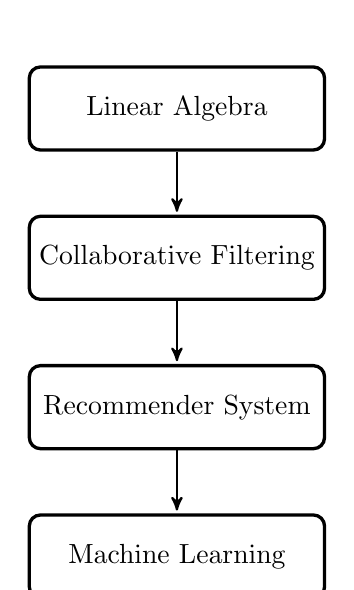
\begin{tikzpicture}
      [node distance=.8cm,
      start chain=1 going below, start chain=2 going below]
      \node[punktchain, join] (la) {Linear Algebra};
      \node[punktchain, join] (cf) {Collaborative Filtering};
      \node[punktchain, join] (rs) {Recommender System};
      \node[punktchain, join] (ml) {Machine Learning};
    \end{tikzpicture}
  \end{center}

  % ----------------------------------------------------------------------------------------

\end{document}
